%!TEX root = ../main.tex
\chapter{Analýza problematiky}
\section{Motivácia}
\paragraph{}
Mobilne zariadenia sa stavaju coraz vacsou sucastou nasich zivotou. Často sú vybavené GPS i mobilným pripojenim, bluetooth, fotoaparatom, NFC scannerom, či inými technológiami. Stali sa moderným švajčiarskym nožíkom spoločnosti. Využívané na pracu, vzdelávanie i zábavu. S prichodom novych techonologii sa vsak stretavame s coraz viac narastajucim problemom. Vďaka nim sa všetky vzdialenosti skracujú. Informácie, miesta, umenie, priatelia, sú na dosah ruky. A tak sa pohyb stáva určitým bonusom k životu vo svete pixelov. Prečo však nevyužiť pixely na tychto šikovných pomôckach aby dostali ludí do pohybu?\\
Mnozstvo skvelych napadov vsak zostava neuskutocnenych kvoli nedostatku času, financnych prostriedkov či znalosti programovania. Preto som sa rozhodol vytvorit framework pre tvorbu GPS online hier. Vdaka, ktoremu by si kazdy clovek mohol spravit vlastny svet neuveritelne jednoduchšie a rýchlejšie ako pri vývoji novej hry. Kde praca na vytvorenie hry sa prenecha nastroju, ktory potrebuje iba nápad.

\section{Svet hier}
\subsection{MMORPG}
Massive multiplayer online role playing game - je typ hry, ktora je zalozena na veľkom pocte hracov hrajucich spolu v hernom svete s prvkami role playing game. Hrac teda hrá za postavu. Prechádza herným svetom. Má určité atribúty, zbrane, schopnosti či rozne iné objekty. Postava pomocou nich získava v tomto svete skúsenosti, peniaze či objekty plnením rôznych úloh či porážaním nepriatelov v boji. 
Medzi najznámejšie, ktoré si môžeme spomenúť patria World of Warcraft, EVE online, Guild Wars. Dennodenne ich hrajú milióny hráčov, ktorý spolupracujú a súperia navzájom.

\begin{figure}[h]
  \centering
  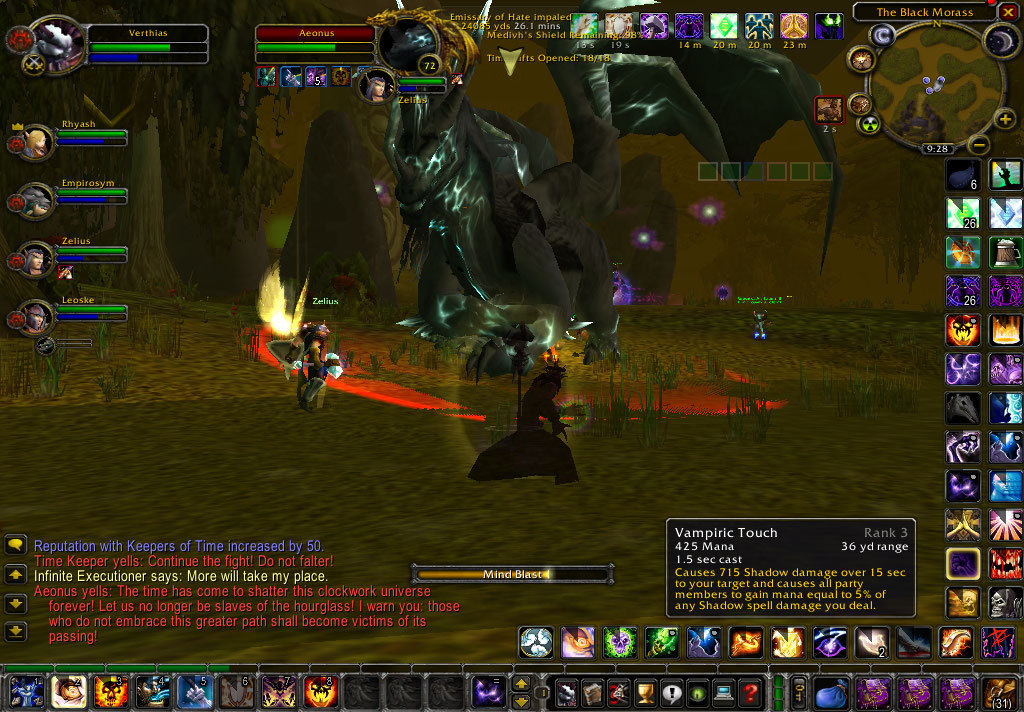
\includegraphics[height=10cm]{mainmatter/imgs/wow.jpg}
  \caption{Počítačová hra World of Warcraft}
  \label{fig:comenius}
\end{figure}

\subsection{Šifrovacie hry}

\subsection{Geocaching}\cite{geocaching} je hra s prvkami turistiky, ktorej cieľom je nájdenie skrytého objektu (kešky). Jedinú informáciu, ktorú hráč má je len poloha tohto schovaného predmetu. Často je potrebné riešiť úlohy, ktorých vyriešením hráč získa súradnice cieľa, ktorý potom môže nájsť presne pomocou GPS navigačeho zariadenia.

\section{Technológie}


\subsection{MVC} alebo model, view, controller architektura založená na rozdelení aplikácie do týchto troch zložiek. Model je tvorený dátami, ktoré reprezentuje v aplikácii a obsahuje tiež hlavnú logiku pre prácu s nimi. View sa stará o vizuálnu stránku, ktorá je ako výsledok prezentovaná používatelovi. Controller spracováva jednotlivé dopyty od používatela a stará sa o interakciu s modelom a view.
\begin{figure}[h]
  \centering
  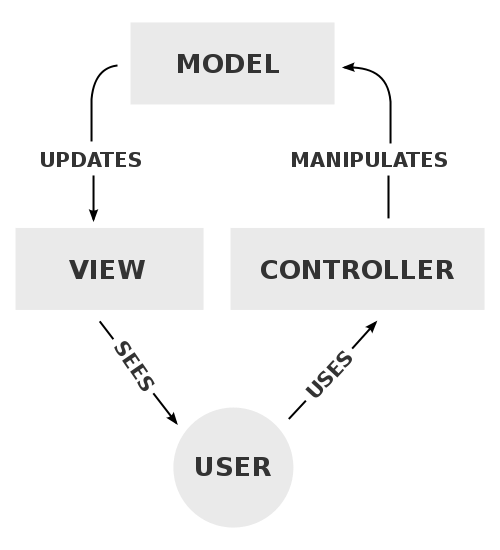
\includegraphics[height=10cm]{mainmatter/imgs/mvc.png}
  \caption{MVC architektúra}
  \label{fig:comenius}
\end{figure}

% \subsection{Android} Na strane klienta je zvolený operačný systém Android od firmy Google. Ktorý sa vačšinou používa práve na mobilných zariadeniach. Oproti konkurenčnému systému iOS od Apple je operačný systém open source. Ďalším argumentom bola politika schvalovania aplikácii a možnosť ich vyvýjať na rôznych operačných systémoch, kde pre android je to možné takmer pod každým operačným systémom. Ďaľšou možnosťou bol Windows Phone, ten však bol zavrhnutý kvôli jeho nižšiemu rozšíreniu \
% Android ma jadro založené na linuxe. Aplikácie možno vývíjať v jazyku Java pomocou Android SDK, ktorý ponúka funkcie na ovládanie zariadenia.


\subsection{Bluetooth} je radiový štandard IEEE 802.15.1, ktorý slúži tiež na bezdotykovú komunikáciu medzi zariadeniami. Bol vytvorený firmou Ericsson v roku 1994. Pomenovaný je podľa dánskeho kráľa s menom Harald Blatand (do angličtiny prelozené ako Bluetooth), ktorému sa podarilo vďaka jeho diplomatickým schopnostiam uzmieriť kmene, ktoré proti sebe bojovali. Podla typu bluetooth vysielačov/prijímačov môžu mať navzajom dosah až po 400metrov. Najčastejšie sú však zariadenia s dosahom 10metrov. S novšími verziami bluetooth je možná rýchlosť prenosu dát až 24 Mbit za sekundu. Často sa používa na jednoduche posielanie dát medzi mobilnými zariadeniami či bezdrotovych slúchadlách. 


\subsection{QR Kody} QR (Quick Response) sú čiarové kódy, v ktorých je uložená informácia. Boli vyvinuté japonskou automobilkou Toyota na rýchle čítanie informácii o tovare nimi označenými. Sú zložené z bielych a čiernych štvorcov usporiadaných v mriežke. Môžu byť vytlačené na papier a prečítané pomocou čítačiek či zariadení, ktoré zosnímajú kód a dokážu ho preložiť spať do pôvodnej informácie.  QR kódy sú často pridávané do reklamných plagátov či videí ako odkazy na produkty výrobcu. Nájdeme ich ale i pri kultúrnych pamiatkach ako ďaľší zdroj informacií. Využitia sú rôzne kedže na relatívne malej ploche dokážu uložit 7089 numerických, 4296 alfanumerických, 2953 binárnych či 1817 kanji znakov\cite{qrcode-about}. QR kódy obsahujú tiež pripravenú opravu chýb pri mierne poškodenom QR kóde a tak je čítačka schopná prečítať informáciu napríklad, keď je kúsok QR kódu prekrytý\cite{qrcode-about}. 

\subsection{NFC} Možno ani netušite, že ste sa už s NFC stretli. Napríklad ak ste platili pri nákupoch pomocou karty bezdotykovo. NFC (Near field communcation) je pomerne mladá technológia, pomocou ktorej môžu zariadenia medzi sebou komunikovať na krátku vzdialenosť (maximálne 20 centimetrov) bezdotykovo. Je potomkom RFID - Rádiofrekvenčných identifikačných kariet a ich čítačiek, ktoré sa spojili v NFC. Takže dokáže komunikovať s obomi i ostatnými zariadeniami, ktoré NFC majú.

\section{Frameworky, knižnice a API}

\subsection{Codeigniter} open sourceovy(OSL) PHP framework. Zakladá si na MVC architektúre avšak necháva volnosť programátorovi. Taktiež ako ďaľšiu z klúčových vlastností pre jeho výber bola jeho rýchlosť\cite{codeigniter-guide}. Bol založený v roku 2006 a je vyvíjaný americkou firmou EllisLab. Jej ďaľším dôležitým prvkom sú tiež knižnice a nástroje, ktoré ulahčujú vývoj aplikacie. Jeho funkcionalitu je možné rozširovať pomocou helperov a rožširovaní tried.

\subsection{jQuery} je veľmi obľúbená\cite{jquery-usage} javascriptová knižnica, ktorá uľahčuje prácu hlavne pri manipulovaní s objektami na stránke. Často sa teda využíva pri tvorbe efektov, či žjednodušovaní vývoja aplikácií využívajúcich javascript. jQuery sa o to všetko snaží pri zachovávaní kompatibility medzi rôznymi internetovými prehliadačmi\cite{jquery-browsers}. Podporuje množstvo rozšírení pomocou pluginov\cite{jquery-plugins}. jQuery je opensource projekt vydavaný pod MIT licenciou. 

\subsection{Bootstrap} je front-endový framework pre tvorbu webových stránok. Je vytvorený pomocou HTML a CSS. Bol založený členmi vývojového tímu Twitteru a v roku 2011 vydaný ako opensource projekt\cite{bootstrap-about}. Obsahuje rôzne šablóny pre dizajn rôznych komponentov na webových stránkach ako sú napríklad gombíky, formy, navigácie. Bootstrap podporuje responzívny design. Responzívne stránky sa teda môžu prispôsobovať pre jednotlivé zariadenia s rôznymi rozlíšeniami obrazoviek. Poslúži nám na vytvorenie moderneho a funkčného designu. Ktorý bude podporovaný medzi rôznymi webovými prehliadačmi.


\subsection{Google maps} je služba od internetového giganta Google pomocou, ktorej zobrazíme mapu réalneho sveta ale i toho fiktívneho - herného. Funguje ako javscriptová, css, html služba, je ktorá má vśak svoje obmedzenie pri používaní zadarmo - 25 000 načítaní za deň\cite{gmaps-usage}.


% \subsection{Google directions} Ďalšia zo služieb, ktorú Google ponúka. Táto sa stará o navigáciu z bodu A do bodu B a poskytuje potrebné informácie pre potrebné pokyny.

\subsection{QR code generator} je na strane serveru jasnou volbou pre jeho množstvo funkcii a parametrov\cite{qrgenerator-functions}, ktoré poskytuje pri tvorbe QR kodov. QR kody budú môcť byť generované užívateľmi a pridané do hry a tak prispievať a vyvíjat obsah do hry.



\subsection{ZBar} je GPL knižnica pre Androidy pomocou, ktorej môžeme skenovať a rozoznávať QR kódy. Vybraná je táto napriek obľúbenej knižnici zxing, ktorá pre svoje použitie sa musí stiahnuť ich aplikácia ktorej sa posiela požiadavok, čo by nebolo veľmi príjemné. ZBar sa teda bude zakomponovaný do našej klientskej android aplikácie\cite{qrreader}.

\subsection{Iconify}


\section{Prehľad existujúcich aplikácií}

\subsection{Nástroje na tvorbu hier}

\subsubsection{Realm Crafter} Je komerčný nástroj na tvorbu MMORPG avšak na počítač. Dá sa pomocou neho relativne jednoducho vytvorit herný svet. Okrem ceny a trošku zložitejšej tvorby sveta sa dajú vytvoriť presvedčivé výsledky. Hlavným problémom je nemožnosť tvorby hier na smartphony využívajucích GPS.

\subsubsection{Rpg Maker} je ďaľší komerčný program, ktorý užívateľom umožňuje vytvárať ich vlastné dvojrozmerné RPG na počítač. Napriek tomu, že herný engine je určený hlavne na tvorbu hier tohto žánru sa v ňom dajú vytvárať aj hry z iných - napríklad adventury\cite{rpg-maker-game}. Obsahuje editor s predrobeným balíkom textúr a obrázkov postavičiek. Používatel však môže pridať i vlastné. 
\cite{rpg-maker}

\subsection{Hry}
\subsubsection{Ingress} Je hra založená tiež na pohybe hráčov v reálnom svete a pomocou mobilných android zariadeni s GPS a internetovým pripojením pohybovaním v hernom svete. Hra je zadarmo a viac strategiou pre tímy. Avšak naším cielom je tvorba podobných hier a s prvkami RPG.


\subsubsection{Shakes\&Fidget} je online hra, ktorú je možné hrať vo webovom prehliadači\cite{sfgame}. Hráč si vytvorí svoju postavu, ktorému môže vybrať rasu a o aký typ bojovníka sa jedná. Postava má rôzne vlastnosti, ktoré si môže vylepšovať. Herné peniaze, veci a skúsenosti získava cez súboje s nepriatelmi a plnením úloh. Herný systém je veľmi podobný tomu, ktorý bude využítý v tejto práci.

\begin{figure}
  \centering
  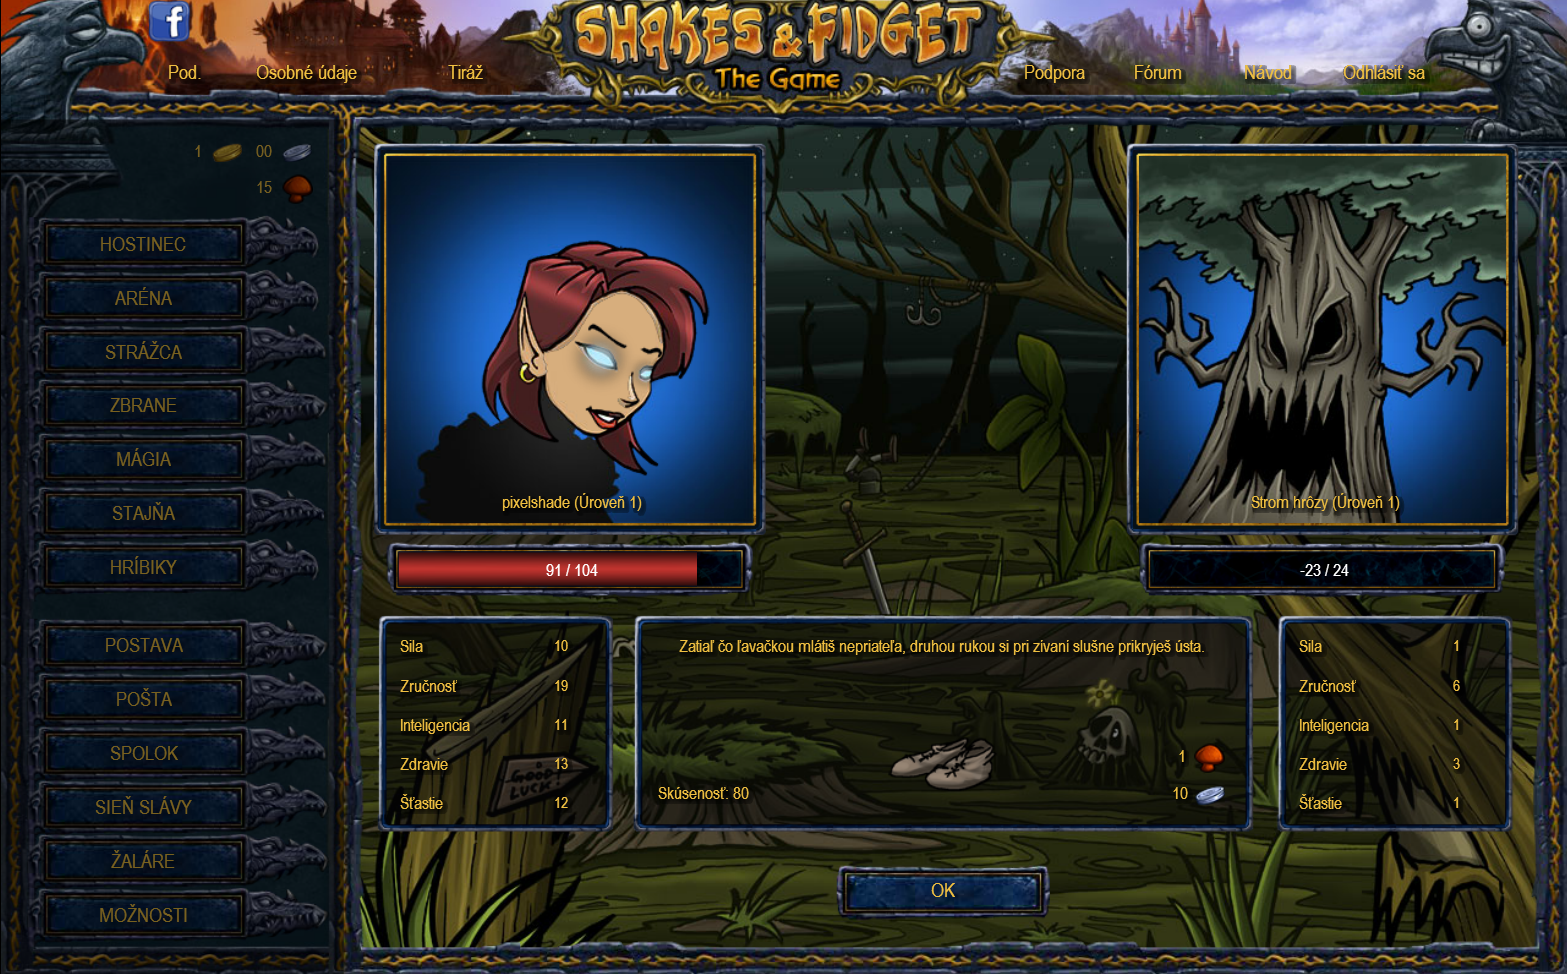
\includegraphics[height=10cm]{mainmatter/imgs/shakes.png}
  \caption{Shakes\&Fidget - súboj postavy s nepriatelom}
  \label{fig:comenius}
\end{figure}


\subsubsection{World of Warcraft} je hlavne MMORPG PC hra, ktorá získala miliony hráčov hlavne pre svoju atmosféru a hrateľnosť. Bola vytvorená firmou Blizzard\cite{wow-blizard}. Hra má klasické črty MMORPG, na rozdiel od Shakes\&Fidget sa však hráč pohybuje so svojou postavou po hernom svete a má omnoho väčšie možnosti interakcie s prostredím\cite{wow-blizard-guide}. 
Výhody
\begin{itemize}
  \item Atmosféra
  \item Grafika 
  \item Hratelnosť \ldots
\end{itemize}
